\documentclass[12pt]{article}
\usepackage{tabularx}
\usepackage{amsmath} 
\usepackage{graphicx}
\usepackage[margin=1in]{geometry}
\usepackage{cite}
\usepackage[final]{hyperref}
\hypersetup{
	colorlinks=true,      
	linkcolor=blue,       
	citecolor=blue,       
	filecolor=magenta,    
	urlcolor=blue         
}
\usepackage{blindtext}
\usepackage{amssymb}
\usepackage{esint}
\usepackage{tikz}
\usepackage{pgfplots}
\usepackage{gensymb}
\usetikzlibrary{datavisualization}
\usetikzlibrary{datavisualization.formats.functions}
\newcommand{\Prho}{.8}%
\newcommand{\Ptheta}{55}%
\newcommand{\Pphi}{60}%
\usepackage{tikz-3dplot}
\newcommand{\uvec}[1]{\boldsymbol{\hat{\textbf{#1}}}}
%++++++++++++++++++++++++++++++++++++++++
\usepackage{empheq}

\newcommand*\widefbox[1]{\fbox{\hspace{2em}#1\hspace{2em}}}

\begin{document}

\usetikzlibrary{scopes}
\def\iangle{35} % Angle of the inclined plane

\def\down{-90}
\def\arcr{0.5cm} % Radius of the arc used to indicate angles


\title{ECE 3030 - HW 1}
\author{Joshua Tensuan - jvt24}
\date{August 27, 2022}
\maketitle


\begin{enumerate}
	\item [1.1]
	\begin{enumerate}
		\item [a.]
		The gradient operator in Cartesian coordinates is given by,
		\[\nabla = \hat x \frac{\partial}{\partial x} + \hat y \frac{\partial}{\partial y} + \hat z \frac{\partial}{\partial z}\]
		Applying the operator to $\phi$,
		\[\nabla \phi = (2ax)\hat x + (2ay )\hat y + (2az)\hat z\]
		\[\boxed{\nabla \phi = (2ax)\hat x + (2ay )\hat y + (2az)\hat z}\]

		\item [b.]
		We know that in cylindrical coordinates,
		\[x^2+y^2=r^2, \; z=z\]
		Substituting these in,
		\[\boxed{\phi(r,\theta, z)=a(r^2+z^2)}\]
		In cylindrical coordinates, the gradient operator is given by,
		\[\nabla = \hat r \frac{\partial}{\partial r}+\hat \theta \frac{1}{r}\frac{\partial}{\partial \theta} + \hat z \frac{\partial}{\partial z}\]
		Applying the operator to $\phi$,
		\[\nabla \phi = (2ar)\hat r + (2az)\hat z\]
		\[\boxed{\nabla \phi = (2ar)\hat r + (2az)\hat z}\]

		\item [c.]
		In spherical coordinates, we know that,
		\[x^2+y^2+z^2= \rho^2\]
		Substituting these in,
		\[\boxed{\phi(r,\theta, \varphi)=a\rho^2}\]
		In spherical coordinates, the gradient operator is given by,
		\[\nabla = \hat \rho \frac{\partial}{\partial \rho}+\hat \theta\frac{1}{\rho}\frac{\partial }{\partial \theta}+ \hat \varphi \frac{1}{\rho\sin(\theta)}\frac{\partial }{\partial \varphi}\]
		Applying the operator to $\phi$,
		\[\nabla \phi = (2a\rho)\hat \rho\]
		\[\boxed{\nabla \phi = (2a\rho)\hat \rho}\]

		\item [d.]
		Use $\nabla \phi$ in Cartesian coordinates given by,
		\[\nabla \phi = (2ax)\hat x + (2ay) \hat y + (2az)\hat z\]
		Applying the divergence operator,
		\[\nabla \cdot \nabla \phi = \frac{\partial}{\partial x}(2ax) + \frac{\partial }{\partial y}(2ay)+\frac{\partial}{\partial z}(2az)=6a\]
		\[\boxed{\nabla^2\phi=\nabla \cdot\nabla \phi=6a}\]
		

	\end{enumerate}

	\item [1.2]
	\begin{enumerate}
		\item [a.]
		\begin{enumerate}
			\item [i.]
			The graph of the vector field is given below.

			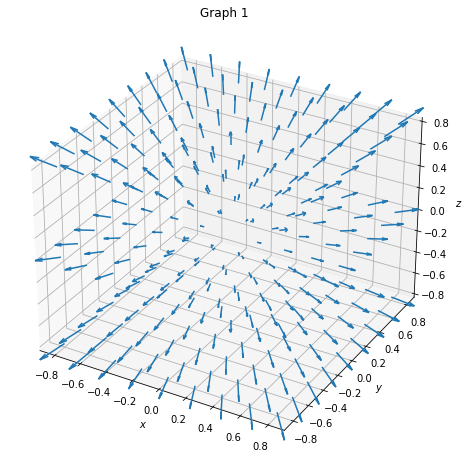
\includegraphics[width = 5in]{images/graph1.png}

			\item [ii.]
			The graph of the vector field is given below.

			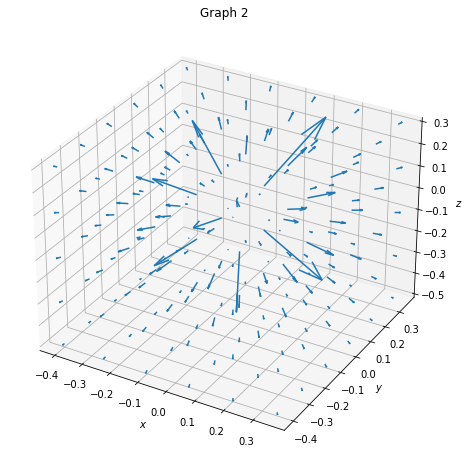
\includegraphics[width = 5in]{images/graph2.png}

			\item [iii.]
			The graph of the vector field is given below.

			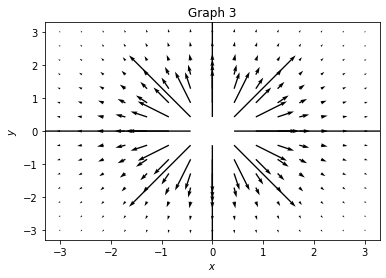
\includegraphics[width = 5in]{images/graph3.png}
		\end{enumerate}

		\item [b.]
		\begin{enumerate}
			\item [i.]
			\[\nabla \cdot \vec F = \frac{\partial}{\partial x}(x)+\frac{\partial }{\partial y}(y)+\frac{\partial}{\partial z}(z)=3\]
			\[\boxed{\nabla \cdot \vec F = 3}\]

			\item [ii.]
			We can convert $\vec F$ into spherical coordinates.
			\[\vec F(\rho, \theta, \varphi)=\left(\frac{\rho\sin(\theta)\cos(\varphi)}{\rho^3}\right)\hat x\]
			\[\vec F = \frac{x}{\rho^3}\hat x + \frac{y}{\rho ^3}\hat y + \frac{z}{\rho ^3}\hat z=\frac{1}{\rho^2}\hat \rho\]
			For a vector with only a $\hat \rho$ component, the divergence of $\vec F$ in spherical coordinates is given by,
			\[\nabla \cdot \vec F =\frac{1}{\rho^2}\frac{\partial}{\partial \rho}(r^2A_{\rho})=\frac{1}{\rho^2}(0)=0\]
			\[\boxed{\nabla \cdot \vec F = 0}\]

			\item [iii.]
			We can convert $\vec F$ into polar coordinates.
			\[\vec F(r, \theta)=\frac{1}{r^2}\hat r\]
			For a vector with only a $\hat r$ component, the divergence of $\vec F$ in polar coordinates is given by,
			\[\nabla \cdot \vec F = \frac{\partial}{\partial r}(F_r)=\frac{\partial}{\partial r}\left(\frac{1}{r^2}\right)=-\frac{2}{r^3}\]
			Using the fact that $r=\sqrt{x^2+y^2}$,
			\[\boxed{\nabla \cdot \vec F = -\frac{2}{(x^2+y^2)^{3/2}}}\]

		\end{enumerate}

		\item [c.]
		\begin{enumerate}
			\item [i.]
			Because divergence is positive, vector field is expanding.

			\item [ii.]
			Because divergence is 0, vector field is not expanding or  contracting.

			\item [iii.]
			Because divergence is negative, vector field is contracting.

		\end{enumerate}


	\end{enumerate}


	\item [1.3]
	\begin{enumerate}
		\item [a.]	
		We can separate the closed surface integral into three separate surfaces via the linearity of the integral operator.
		Let surface 1 denote the top face ($+z$) of the cylinder, surface 2 denote the lateral face of the cylinder, and surface 3 denote the bottom face ($-z$) of the cylinder.
		\[\oiint \vec F \cdot d\vec A = \iint_{S_1}\vec F \cdot d\vec A + \iint_{S_2} \vec F \cdot d\vec A + \iint_{S_3} \vec F \cdot d\vec A\]
		We can convert $\vec F$ to cylindrical coordinates for ease of calculation via,
		\[\vec F = (x\hat x + y\hat y + z^2\hat z)=r\hat r + z^2\hat z\]
		Starting by evaluating $\iint_{S_1}\vec F \cdot d\vec A$, 
		\[\iint_{S_1}\vec F \cdot d\vec A = \iint_{S_1}\vec F \cdot \vec N \: dr \: d\theta\]
		The parameterization of the surface, $G(r,\theta)$, is given on $r:(0,d/2)$ and $\theta:(0,2\pi)$ as,
		\[G(r,\theta)=\left\langle r\cos(\theta), r\sin(\theta), \frac{L}{2}\right\rangle\]
		Finding the normal vector,
		\[\frac{\partial G}{\partial r}=\langle \cos(\theta),\sin(\theta), 0\rangle\]
		\[\frac{\partial G}{\partial \theta}=\langle -r\sin(\theta),r \cos(\theta),0 \rangle\]
		\[\vec N = \frac{\partial G}{\partial r}\times \frac{\partial G}{\partial \theta}=r\hat z\]
		Substituting this in,
		\[\int_0^{2\pi}\int_0^{d/2}\vec F \cdot \vec N \: dr \: d\theta\]
		\[\vec F \cdot \vec N = rz^2\]
		Considering $z=L/2$,
		\[\vec F \cdot \vec N = \frac{rL^2}{4}\]
		Substituting this into the integral,
		\[\int_0^{2\pi}\int_0^{d/2}\frac{rL^2}{4}\:dr\:d\theta\]
		Evaluating the integral,
		\[=\int_0^{2\pi}\left[\frac{r^2L^2}{8}\right]_0^{d/2}\:d\theta=2\pi\left(\frac{d^2L^2}{32}\right)\]
		\[=\pi \frac{d^2L^2}{16}\]
		Evaluating the $S_3$ surface integral,
		Because $S_3$ is the same surface as $S_1$ but reflected across the $xy$-plane, we know that we will have the same vector $N$ but multiplied by $-1$.
		Substituting this in,
		\[\iint_{S_3}\vec F\cdot d\vec A=\int_0^{2\pi}\int_0^{d/2}-rz^2\:dr\:d\theta\]
		Considering $z=-L/2$,
		\[\iint_{S_3}\vec F\cdot d\vec A=\int_0^{2\pi}\int_0^{d/2}-\frac{rL^2}{4}\:dr\:d\theta\]
		This is equal to $-\iint_{S_1}\vec F \cdot d\vec A$, and thus,
		\[\iint_{S_1}\vec F \cdot d\vec A + \iint_{S_3}\vec F \cdot d\vec A = 0\]
		Finally, computing $\iint_{S_2}\vec F \cdot d\vec A$,
		\[\iint_{S_2}\vec F \cdot d\vec A = \iint_{S_2}\vec F \cdot \vec N \: dr\:d\theta\]
		The parameterization of the surface, $G(z,\theta)$, is given on $z:(-L/2,L/2)$ and $\theta:(0,2\pi)$ as,
		\[G(z, \theta)=\left\langle \frac{d}{2}\cos(\theta),\frac{d}{2}\sin(\theta),z\right\rangle\]
		Finding the normal vector,
		\[\frac{\partial G}{\partial z}=\langle 0, 0, 1\rangle\]
		\[\frac{\partial G}{\partial \theta} = \left\langle -\frac{d}{2}\sin(\theta),\frac{d}{2}\cos(\theta),0 \right\rangle\]
		\[\vec N = \frac{\partial G}{\partial z}\times \frac{\partial G}{\partial \theta}=\begin{vmatrix}
			\hat x & \hat y & \hat z \\ 
			0 & 0 & 1 \\ 
			-\frac{d}{2}\sin(\theta) & \frac{d}{2}\cos(\theta) & 0	
		\end{vmatrix}\]
		Computing this and orienting the boundary correctly, we find that,
		\[\vec N = \frac{d}{2}\cos(\theta)\hat x + \frac{d}{2}\sin(\theta)\hat y=\frac{d}{2}\hat r\]
		$\vec F$ is given by,
		\[\vec F = x\hat x + y\hat y+z^2\hat z\]
		At the boundary of a lateral cross-section of the cylinder, $\sqrt{x^2+y^2}=d/2$.
		Thus, we can reduce $\vec F$ to,
		\[\vec F=\frac{d}{2}\hat r\]
		Thus, $\vec F \cdot \vec N$ is given by,
		\[\vec F \cdot \vec N = \frac{d^2}{4}\]
		Thus,
		\[\iint_{S_2}\vec F \cdot d\vec A = \int_0^{2\pi}\int_{-L/2}^{L/2}\frac{d^2}{4}\:dz\:d\theta=\frac{Ld^2}{2}\pi\]
		Thus, adding up all the individual surface integrals,
		\[\boxed{\oiint \vec F \cdot d\vec A =\frac{Ld^2}{2}\pi}\]

		\item [b.]
		Computing the divergence,
		\[\nabla \cdot \vec F = \frac{\partial F_x}{\partial x}+\frac{\partial F_y}{\partial y}+\frac{\partial F_z}{\partial z}=2+2z\]
		\[\boxed{\nabla \cdot \vec F = 2+2z}\]

		\item [c.]
		\[\iiint \nabla \cdot \vec F \: dV\]
		Using cylindrical coordinates,
		\[\int_0^{2\pi}\int_0^{d/2}\int_{-L/2}^{L/2}r(2+2z)\:dz\:dr\:d\theta\]
		\[\int_0^{2\pi}\int_0^{d/2}r\left[2z+z^2\right]_{-L/2}^{L/2}\:dr\:d\theta\]
		\[\int_0^{2\pi}\int_0^{d/2}2Lr\:dr\:d\theta\]
		\[\int_0^{2\pi}\frac{Ld^2}{4}\:d\theta\]
		\[\iiint \nabla \cdot \vec F \: dV = \frac{Ld^2}{2}\pi\]
		\[\boxed{\iiint \nabla \cdot \vec F \: dV = \frac{Ld^2}{2}\pi}\]

		\item [d.]
		Via divergence theorem, we know that,
		\[\oiint \vec F \cdot d\vec A = \iiint \nabla \cdot \vec F \: dV\]
		From part a, we calculated,
		\[\oiint \vec F \cdot d\vec A =\frac{Ld^2}{2}\pi\]
		From part c, we calculated,
		\[\iiint \nabla \cdot \vec F \: dV = \frac{Ld^2}{2}\pi\]
		These two values are identically equal.
		Thus, divergence theorem is verified.
		\[\boxed{\text{Q.E.D}}\]

	\end{enumerate}

	\item [1.4]
	\begin{enumerate}
		\item [a.]
		Evaluating the line integral,
		\[\oint \vec F \cdot d\vec s\]
		\[d\vec s = -\sin(\varphi)dx\:\hat x + \cos(\varphi)dy\:\hat y\]
		In cylindrical coordinates,
		\[d\vec s = r \:d\varphi\:\hat \varphi\]
		At $z=0$, and along the given contour ($r=a$), $\vec F = a\hat \varphi + \hat z$
		\[\vec F \cdot d\vec s = a^2\:d\varphi\]
		\[\oint \vec F \cdot d\vec s = \int_0^{2\pi}a^2\:d\varphi=2\pi a^2\]
		\[\boxed{2\pi a^2}\]

		\item [b.]
		In cylindrical coordinates, the curl operator is given by,
		\[\nabla \times \vec A= \left(\frac{1}{r}\frac{\partial A_z}{\partial \varphi}-\frac{\partial A_\varphi}{\partial z}\right)\hat r+\left(\frac{\partial A_r}{\partial z}-\frac{\partial A_z}{\partial r}\right)\hat \varphi + \left(\frac{1}{r}\frac{\partial}{\partial r}(rA_\varphi)-\frac{1}{r}\frac{\partial A_r}{\partial \varphi}\right)\hat z\]
		Inputting $\vec F$,
		\[\nabla \times \vec F = \left(\frac{1}{r}(0)-0\right)\hat r + \left(2-0\right)\hat \varphi + \left(\frac{1}{r}\frac{\partial}{\partial r}(r^2)-\frac{1}{r}(0)\right)\hat z\]
		\[\nabla \times \vec F = 2\hat \varphi + 2\hat z\]
		\[\boxed{\nabla \times \vec F = 2\hat \varphi + 2 \hat z}\]

		\item [c.]
		We can parametrize the surface over $r:(0,a)$ and $\varphi:(0,2\pi)$ as,
		\[G(r,\varphi)=\left\langle r\cos(\varphi), r\sin(\varphi), 0\right\rangle\]
		Finding the normal vector,
		\[N=\frac{\partial G}{\partial r}\times \frac{\partial G}{\partial \varphi}\]
		\[\frac{\partial G}{\partial r}=\langle \cos(\varphi),\sin(\varphi, 0 \rangle)\]
		\[\frac{\partial G}{\partial \varphi}=\langle -r\sin(\varphi), r\cos(\varphi), 0\rangle\]
		\[N = r\hat z\]
		Substituting this into the flux integral,
		\[\iint (\nabla \times \vec F)\cdot d\vec A = \iint (\nabla \times \vec F) \cdot \vec N \: dr \: d\varphi\]
		\[(\nabla \times \vec F)\cdot \vec N = 2r\]
		Substituting this into the integral,
		\[\int_0^{2\pi}\int_0^a 2r \: dr \: d\varphi = 2\pi a^2\]
		\[\boxed{2\pi a^2}\]

		\item [d.]
		Via Stokes theorem, we know that,
		\[\iint(\nabla \times \vec F)\cdot d\vec A = \oint \vec F \cdot d\vec s\]
		From part a, we calculated,
		\[\oint \vec F \cdot d\vec s = 2\pi a^2\]
		From part c, we calculated,
		\[\iint (\nabla \times \vec F)\cdot d\vec A = 2\pi a^2\]
		These two values are identically equal.
		Thus, Stokes theorem is verified.

		\item [e.]
		By Stokes theorem, we know that,
		\[\oint \vec F \cdot d\vec s = \iint_S (\nabla \times \vec F)\cdot d\vec A\]
		where surface $S$ corresponds to any surface with a boundary corresponding to the closed loop that the line integral is taken over.
		Because the surface in the prompt has the same exact boundary as the surface in part c, they will correspond to the same line integral by Stokes theorem.
		Thus, the flux integral is given by,
		\[\boxed{2\pi a^2}\]




	\end{enumerate}

	\item [1.5]
	\begin{enumerate}
		\item [a.]
		We can take a proof by contradiction to demonstrate this.
		Without loss of generality (works if we assume $-z$-direction as well), suppose there is a component of the electric field in the $+z$-direction.
		Rotate the entire system by $\pi$ about the $y$-axis (identical to performing a mirror reflection about $xy$-plane).
		If we again assume the original coordinate system, there will now be a component of the electric field in the $-z$-direction.
		However, due to the symmetry of the wire, the system should be identically equal.
		This creates a contradiction in the value of the electric field, and thus, there cannot be a component of the electric field in the $\pm z$-direction.
		\[\boxed{\text{Q.E.D}}\]

		\item [b.]
		We can again prove this via contradiction.
		Without loss of generality (works if we assume $-\hat \phi$-direction as well), suppose there is a component of the electric field in the $+\hat \phi$-direction.
		Rotate the  entire system by $\pi$ about the $y$-axis (identical to performing a mirror reflection about $xy$-plane).
		If we again assume the original coordinate system, there will now be a component of the electric field in the $-\hat \phi$-direction.
		However, due to the symmetry of the wire, the system should be identically equal.
		This creates a contradiction in the value of the electric field, and thus, there cannot be a component of the electric field in the $\pm \hat \phi$-direction.
		\[\boxed{\text{Q.E.D}}\]

		\item [c.]
		Form a Gaussian cylinder concentric to the line charge.
		Because there are no components in the $\pm z$-direction as proved by part a, we know that there will be no electric field flux through the top and bottom faces of the cylinder.
		Additionally from part b, we know that there will be no electric field in the $\pm \hat \phi$-direction.
		Thus, the only electric field can point radially outwards from the Gaussian cylinder.
		We can then simplify Gauss' Law to,
		\[\iint \epsilon_0\vec E \cdot d\vec A = Q_{\mathrm{enc}}\]
		\[\epsilon_0E_rA = \lambda l\]
		where $l$ is the length of the Gaussian cylinder.
		Through some algebraic manipulation,
		\[\epsilon_0E_r2\pi rl = \lambda l \to E_r = \frac{\lambda}{\epsilon_0 2\pi r}\]
		\[\boxed{\vec E = \frac{\lambda}{\epsilon_02\pi r}\hat r}\]

		
	\end{enumerate}

	
\end{enumerate}

		

\end{document}
